\chapter{حيود فراونهوفر والترشيح المكاني}\label{ch:b2:diffraction}

حدّق في مصباح شارع من الفرجة بين إصبعين فيمتد
المصباح شريطًا من الهدب؛ وانظر إلى نجم في أدقّ
مقراب فلا ترى نقطة بل قرصًا صغيرًا تحفّه دوائر
خافتة. فالضوء العابر فتحةً ينتشر --- وكلما ضاقت
الفتحة اتسع الانتشار --- ولا تستطيع عدسة أن تجمّعه
أضيق مما يسمح به هذا الانتشار. وهذا هو \emph{\omterm{def:b2:diffraction:huygens}{الحيود}}، وهو سبب
عجز المجهر عن رؤية فيروس، ونموّ قدرة تمييز المقراب
مع قطره، وعجز حزمة الليزر عن البقاء متوازية. وهذا الفصل
يحسب نقش \omterm{def:b2:diffraction:huygens}{حيود} فتحة في الحقل البعيد، والحدّ
الذي يضعه على كل أداة بصرية، وكيف يجتمع مع
التداخل، والفكرة --- فكرة آبي --- التي تجعل من المستوي البؤري
للعدسة موضعًا يمكن فيه ترشيح صورة.

\section{مبدأ هويغنس--فرينل ونظام فراونهوفر}

\begin{definition}[مبدأ هويغنس--فرينل]\label{def:b2:diffraction:huygens}
\index{مبدأ هويغنس--فرينل}\index{حيود}\index{حيود فراونهوفر}
كل نقطة من \omterm{def:b2:scalar-light-model:path}{جبهة موجة} (أو من فتحة تضيئها موجة) تعمل
منبعًا ثانويًّا يصدر موجيرة كروية، على طور الموجة
هناك؛ والموجة وراءها مجموع الموجيرات المترابط. ومن أجل
فتحة $\Sigma$ تضيئها موجة مستوية سعتها $a$، تكون السعة
البالغة نقطة بعيدة $\underline s(M) = K\iint_\Sigma\eu^{-\iu\varphi(P, M)}\dd S$، حيث
$\varphi(P, M)$ طور المسير من نقطة الفتحة $P$ إلى $M$
(و $K$ ثابت). و\emph{حيود فراونهوفر} (أي حيود الحقل البعيد) هو الحالة
التي تكون فيها $M$ في اللانهاية --- أو في المستوي البؤري لعدسة --- بحيث
تكون الأشعة من نقاط الفتحة كلها نحو $M$ متوازية، في
الجهة $\vect u$، ويكون
\[
\varphi(P, M) = \varphi_0 - \frac{2\pi}\lambda\,\vect{OP}\cdot\vect u , \qquad
\underline s(\vect u) \propto \iint_\Sigma\eu^{\iu(2\pi/\lambda)\vect{OP}\cdot\vect u}\dd S .
\]
ويُرصَد النقش في اللانهاية، أو عند بؤرة $F'$ عدسة،
حيث تنطبق الجهة $\vect u$ ذات الزاويتين الصغيرتين $(\alpha, \beta)$ على
النقطة $(f\alpha, f\beta)$.
\end{definition}
\admitted

\begin{remark}[متى يكون البعد كافيًا؟]\label{rem:b2:diffraction:fresnelnumber}
\index{عدد فرينل}
من أجل فتحة حجمها $D$ يُنظر إليها على البعد $L$ من دون عدسة، تكون
الأشعة متوازية كفاية حين يكون الحدّ التربيعي في
\cref{exo:b2:scalar-light-model:12} مهمَلًا، $D^2/L \ll \lambda$ ---
أي \emph{\omterm{rem:b2:diffraction:fresnelnumber}{عدد فرينل}} $D^2/\lambda L \ll 1$. وشقّ \qty{0.1}{mm} عند
\qty{500}{nm} يحتاج إلى $L \gg \qty{2}{cm}$؛ وفتحة \qty{1}{cm} تحتاج إلى $L \gg \qty{200}{m}$ ---
ومن هنا العدسة، التي تجلب اللانهاية إلى مستويها البؤري. وأما في ما هو أقرب
(أي \omterm{def:b2:diffraction:huygens}{حيود} فرينل) فالنقوش أعقد؛ ولظلّ
حرف مستقيم، مثلًا، هدب على جانبه المضاء.
\end{remark}

\section{الشقّ الوحيد والفتحة الدائرية}

\begin{proposition}[الحيود على شقّ]\label{prop:b2:diffraction:slit}
\index{حيود الشقّ الوحيد}\index{تابع الجيب المقسوم}
شقّ عرضه $b$ (طويل وفق $y$) مضاء عند الورود الناظمي يرسل في
الجهة $\theta$ (في المستوي العمودي على الشقّ)
الشدة
\[
I(\theta) = I_0\,\operatorname{sinc}^2\Bigl(\frac{\pi b\sin\theta}\lambda\Bigr) , \qquad \operatorname{sinc}x = \frac{\sin x}x :
\]
أي موضع عظم مركزي مضيء نصف عرضه الزاوي $\lambda/b$ (وأول صفرين عند
$\sin\theta = \pm\lambda/b$)، يحوي $90\%$ من الضوء، ومواضع عظم ثانوية
عند نحو $\sin\theta = \pm1.43\lambda/b$، و $\pm2.46\lambda/b$، \dots، وشدّاتها
النسبية $4.7\%$، و $1.6\%$، \dots --- وكلما ضاق الشقّ اتسع
النقش. وفي المستوي البؤري لعدسة بعدها البؤري $f$ يكون
عرض موضع العظم المركزي $2\lambda f/b$.
\end{proposition}

\begin{proof}
$\underline s(\theta) \propto \int_{-b/2}^{b/2}\eu^{\iu kx\sin\theta}\dd x = b\,\operatorname{sinc}(kb\sin\theta/2)$
مع $k = 2\pi/\lambda$؛ ثم ربّع. والأصفار حيث $b\sin\theta = m\lambda$، و $m \ne 0$: إذ
تتلاشى عندئذ موجيرات نصفي الشقّ مثنى مثنى.
\end{proof}

\begin{omfigure}
\begin{tikzpicture}[font=\small, x=1cm, y=1cm, >=Stealth]
  \begin{scope}
    \draw[thick] (0,-2) -- (0,-0.5) (0,0.5) -- (0,2);
    \draw[<->] (-0.35,-0.5) -- (-0.35,0.5) node[midway, left, font=\footnotesize] {$b$};
    \foreach \y in {-1.6,-0.9,-0.2,0.5,1.2} \draw[omDef, ->] (-2.2,\y) -- (-0.1,\y);
    \foreach \y in {-0.4,-0.2,0,0.2,0.4} \draw[omThm, thick, ->] (0.1,\y) -- (2.4,{\y+1.0});
    \draw[dashed] (0.1,0) -- (2.6,0); \draw (1.4,0) arc[start angle=0, end angle=23.5, radius=1.4]; \node[font=\footnotesize] at (1.7,0.28) {$\theta$};
    \node[font=\footnotesize] at (1.2,-1.6) {$b\sin\theta = \lambda$: أول صفر};
  \end{scope}
  \begin{scope}[xshift=8.6cm]
    \begin{axis}[omaxis, axis x line=bottom, axis y line=left, width=6.4cm, height=4.4cm, at={(0,-2.0cm)},
        xlabel={$b\sin\theta/\lambda$}, ylabel={$I/I_0$}, xmin=-3.2, xmax=3.2, ymin=0, ymax=1.1, xtick={-3,-2,-1,0,1,2,3}, ytick={0.5,1}, samples=400,
        xlabel style={at={(axis description cs:0.5,-0.14)}, anchor=north},
        ylabel style={at={(axis description cs:-0.1,0.5)}, rotate=90, anchor=south}]
      \addplot[omDef, thick, domain=-3.2:3.2] {(sin(deg(pi*x))/(pi*x+1e-9))^2};
    \end{axis}
  \end{scope}
\end{tikzpicture}

{\small على اليسار: موجيرات الشقّ، مجموعة في الجهة
$\theta$. وعلى اليمين: نقش فراونهوفر للشقّ، $\operatorname{sinc}^2$: أي
فصّ مركزي عرضه ضعف الآخرين وأشدّ سطوعًا بكثير.}
\end{omfigure}

\begin{proposition}[الفتحة الدائرية؛ قرص إيري]\label{prop:b2:diffraction:airy}
\index{قرص إيري}\index{معيار رايلي (التمييز)}\index{قدرة التمييز (أداة)}
فتحة دائرية قطرها $D$ تعطي قرصًا مضيئًا مركزيًّا، هو
\emph{\omterm{prop:b2:diffraction:airy}{قرص إيري}}، تحيط به حلقات خافتة؛ وأول حلقة مظلمة عند
\[
\sin\theta = 1.22\,\frac\lambda D ,
\]
ويحمل القرص $84\%$ من الضوء. وكل أداة
حدقة دخولها قطرها $D$ --- العين، وآلة التصوير، والمقراب، وشيئية
المجهر --- تحوّل منبعًا نقطيًّا إلى \omterm{prop:b2:diffraction:airy}{قرص إيري} بهذا نصف القطر
الزاوي؛ وتُفصَل نقطتان \emph{تمييزًا} (بمعيار رايلي) إذا تجاوز
فصلهما الزاوي $1.22\lambda/D$: وهي قدرة تمييز
الأداة.
\end{proposition}
\admitted

\begin{example}[العين والمقراب والمجهر]\label{ex:b2:diffraction:instruments}
العين ($D = \qty{3}{mm}$، $\lambda = \qty{550}{nm}$): $1.22\lambda/D = \qty{2.2e-4}{rad}$، أي نحو
\qty{45}{''} --- أي تفصيل \qty{1}{mm} على \qty{4}{m}، وهو فعلًا نحو
حدّة العين الجيدة: فقد لاءم التطور خلايا الشبكية مع
حدّ \omterm{def:b2:diffraction:huygens}{الحيود}. ومقراب \qty{2.4}{m}: \qty{0.06}{''}، أي أحسن بألف مرة،
إن سمح الجوّ (وهو لا يسمح، من الأرض:
\qty{1}{''} من "الرؤية"، ومن هنا المقاريب الفضائية والبصريات التكيفية). وطبق
راديوي \qty{100}{m} عند $\lambda = \qty{21}{cm}$: \qty{9}{'}، أي أسوأ من العين؛
ومقاييس التداخل عبر القارات تستعيد التمييز. وشيئية
مجهر زاوية فتحتها $\alpha$ تميّز $0.61\lambda/n\sin\alpha$
--- أي نحو \qty{0.2}{\micro m} في المرئي، مهما كان التكبير: وهو
الحدّ الذي ساق المجهرية إلى الإلكترونات وإلى الأشعة السينية.
\end{example}

\begin{omfigure}
\begin{tikzpicture}[font=\small, x=1cm, y=1cm]
  \begin{scope}
    \foreach \r/\g in {1.5/85, 1.25/70, 1.0/50, 0.8/25, 0.6/5, 0.45/40, 0.3/70, 0.15/95} {
      \fill[black!\g] (0,0) circle (\r);
    }
    \node[font=\footnotesize] at (0,-1.9) {نقش إيري لنجم واحد};
  \end{scope}
  \begin{scope}[xshift=4.2cm]
    \foreach \r/\g in {0.8/25, 0.6/5, 0.45/40, 0.3/70, 0.15/95} {
      \fill[black!\g] (-0.45,0) circle (\r);
    }
    \foreach \r/\g in {0.8/25, 0.6/5, 0.45/40, 0.3/70, 0.15/95} {
      \fill[black!\g, opacity=0.6] (0.45,0) circle (\r);
    }
    \node[font=\footnotesize] at (0,-1.9) {نجمان عند حدّ رايلي};
  \end{scope}
  \begin{scope}[xshift=9.6cm]
    \begin{axis}[omaxis, axis x line=bottom, axis y line=left, width=5.4cm, height=4.0cm, at={(0,-1.8cm)},
        xlabel={$\theta D/\lambda$}, ylabel={$I$}, xmin=-2.5, xmax=3.5, ymin=0, ymax=1.5, xtick={-1.22,0,1.22,2.44}, xticklabels={$-1.22$,$0$,$1.22$,$2.44$}, ytick=\empty, samples=300,
        xlabel style={at={(axis description cs:0.5,-0.14)}, anchor=north},
        ylabel style={at={(axis description cs:-0.06,0.5)}, rotate=90, anchor=south}]
      \addplot[omDef, thick, domain=-2.5:3.5] {(sin(deg(pi*x/1.22))/(pi*x/1.22+1e-9))^2};
      \addplot[omThm, thick, domain=-2.5:3.5] {(sin(deg(pi*(x-1.22)/1.22))/(pi*(x-1.22)/1.22+1e-9))^2};
    \end{axis}
  \end{scope}
\end{tikzpicture}

{\small على اليسار وفي الوسط: \omterm{prop:b2:diffraction:airy}{قرص إيري} لمنبع نقطي، ومنبعان
عند حدّ رايلي --- أي مركز أحدهما على أول حلقة مظلمة
للآخر. وعلى اليمين: مقطعاهما (مرسومين بأشكال $\operatorname{sinc}^2$)،
يفصل بينهما $1.22\lambda/D$.}
\end{omfigure}

\section{الحيود والتداخل معًا}

\begin{proposition}[شقّا يونغ ذوا العرض المنتهي؛ غلاف الشبكة]\label{prop:b2:diffraction:combined}
\index{غلاف (حيود)}\index{الرتب الغائبة}
شقّان عرض كل منهما $b$ ويبعد مركزاهما $a$ يعطيان
\[
I(\theta) = 4I_0\,\operatorname{sinc}^2\Bigl(\frac{\pi b\sin\theta}\lambda\Bigr)\cos^2\Bigl(\frac{\pi a\sin\theta}\lambda\Bigr) :
\]
أي هدب يونغ (وتباعدها $\lambda/a$ بدلالة $\sin\theta$) تحت غلاف
الشقّ الوحيد (وعرضه $2\lambda/b$)؛ ويملأ $a/b$ هدبةً الفصَّ المركزي، وتكون
الهدب عند $a\sin\theta = p\lambda$ التي تقع على صفر من أصفار الغلاف
($b\sin\theta = m\lambda$) \emph{غائبة}. وشبكة من $N$ شقًّا عرض كل منها
$b$ لها كذلك مواضع عظم رئيسية يعدّلها الغلاف نفسه ---
وهو ما يميله توجيه \cref{ch:b2:gratings} نحو الرتبة المستعملة.
\end{proposition}

\begin{proof}
ينقسم تكامل الفتحة إلى مجموع على الشقّين لتكامل
واحد مزاح بمقدار $\pm a/2$: $\underline s \propto b\,\operatorname{sinc}(\pi b\sin\theta/\lambda)
\times2\cos(\pi a\sin\theta/\lambda)$. ومن أجل $N$ شقًّا يكون العامل الثاني
مجموع $N$ موجة.
\end{proof}

\begin{omfigure}
\begin{tikzpicture}
\begin{axis}[omaxis, axis x line=bottom, axis y line=left, width=13.6cm, height=4.6cm,
    xlabel={$a\sin\theta/\lambda$}, ylabel={$I/4I_0$}, xmin=-9, xmax=9, ymin=0, ymax=1.1, xtick={-8,-4,0,4,8}, ytick={0.5,1}, samples=1200,
    xlabel style={at={(axis description cs:0.5,-0.12)}, anchor=north},
    ylabel style={at={(axis description cs:-0.04,0.5)}, rotate=90, anchor=south}]
  \addplot[omDef, thick, domain=-9:9] {(sin(deg(pi*x/4))/(pi*x/4+1e-9))^2*cos(deg(pi*x))^2};
  \addplot[omThm, thick, dashed, domain=-9:9] {(sin(deg(pi*x/4))/(pi*x/4+1e-9))^2};
\end{axis}
\end{tikzpicture}

{\small شقّان مع $a = 4b$: هدب يونغ تحت غلاف الشقّ
الوحيد (بالخط المتقطع)؛ وهدب الرتبة الرابعة تقع على أصفار الغلاف
فتغيب.}
\end{omfigure}

\section{مستوي فورييه والترشيح المكاني}

\begin{proposition}[العدسة محلِّلًا لفورييه]\label{prop:b2:diffraction:fourier}
\index{مستوي فورييه}\index{تواتر مكاني}\index{ترشيح مكاني}\index{نظرية آبي}
شفيفة نفاذيتها $t(x, y)$ في المستوي البؤري الأمامي
لعدسة، مضاءة بموجة مستوية، تعطي في المستوي البؤري الخلفي
السعة
\[
\underline s(X, Y) \propto \iint t(x, y)\,\eu^{-\iu2\pi(xX + yY)/\lambda f}\dd x\,\dd y
\]
--- أي تحويل فورييه الثنائي البعد لها، وكل نقطة $(X, Y)$ من
\emph{\omterm{prop:b2:diffraction:fourier}{مستوي فورييه}} تجمع الضوء المحيد عند الزاويتين
$(X/f, Y/f)$، أي \emph{التواترين المكانيين} $(X/\lambda f, Y/\lambda f)$ في
الجسم: فالتفاصيل الدقيقة (أي التواترات العالية) بعيدة عن المحور، والخشنة
قريبة منه. وتعيد عدسة ثانية تكوين الصورة من ذلك المستوي؛ وكل ما
يُحجَب أو يُبدَّل هناك يُرشَّح من الصورة
(أي \emph{\omterm{prop:b2:diffraction:fourier}{الترشيح المكاني}}، وهي \omterm{prop:b2:diffraction:fourier}{نظرية آبي} في المجهر): فثقب دبوس
على المحور لا يبقي إلا التواترات المنخفضة (فيملّس، وينظّف
حزمة ليزر)؛ وحاجب على المحور يزيل الخلفية المنتظمة ويبقي
الحروف (أي الحقل المظلم، والتصوير الخطّي)؛ وصفيحة ربع موجة على
المحور تحوّل الأجسام الطورية، وهي غير مرئية بغير ذلك، إلى تباين شدة
(أي تباين الطور، لزرنيكه).
\end{proposition}

\begin{proof}[تبرير]
في تكامل فراونهوفر، $\vect{OP}\cdot\vect u = x\alpha + y\beta$ مع
الجهة المنطبقة على $(X, Y) = (f\alpha, f\beta)$؛ والنفاذية توزن
كل منبع ثانوي. (وأما تحويل فورييه نفسه فيُدرَس في
مجلد رياضيات السنة الثالثة؛ وهو هنا اسم هذا التكامل لا غير.)
ومن أجل جسم دوري دوره $d$ يكون التحويل مجموعة رتب
الشبكة عند $X = p\lambda f/d$: فلا تستطيع الصورة إظهار الدور إلا إذا مرّت
الرتبتان $\pm1$ على الأقل عبر العدسة --- وهو شرط آبي، وهو
حدّ تمييز المجهر من جديد.
\end{proof}

\begin{omfigure}
\begin{tikzpicture}[font=\small, x=1cm, y=1cm, >=Stealth]
  \draw[omDef, thick, ->] (-5.6,0.8) -- (-4.6,0.8); \draw[omDef, thick, ->] (-5.6,0) -- (-4.6,0); \draw[omDef, thick, ->] (-5.6,-0.8) -- (-4.6,-0.8);
  \draw[thick, fill=omExo!20] (-4.4,-1.4) rectangle (-4.3,1.4); \node[font=\footnotesize] at (-4.35,-1.75) {الجسم $t(x, y)$};
  \draw[thick, fill=omExo!20] (-2.4,0) ellipse (0.2 and 1.5); \node[font=\footnotesize] at (-2.4,-1.85) {$L_1$};
  \draw[thick] (0,-1.4) -- (0,1.4); \fill[omThm] (0,0) circle (2pt); \fill[omThm] (0,0.7) circle (1.5pt); \fill[omThm] (0,-0.7) circle (1.5pt);
  \node[font=\footnotesize] at (0,-1.75) {مستوي فورييه};
  \draw[thick, fill=omExo!20] (2.4,0) ellipse (0.2 and 1.5); \node[font=\footnotesize] at (2.4,-1.85) {$L_2$};
  \draw[thick, fill=omExo!20] (4.3,-1.4) rectangle (4.4,1.4); \node[font=\footnotesize] at (4.35,-1.75) {الصورة};
  \draw[omThm] (-4.35,0.6) -- (-2.4,1.0) -- (0,0.7) -- (2.4,0.4) -- (4.35,-0.6);
  \draw[omThm] (-4.35,-0.6) -- (-2.4,-1.0) -- (0,-0.7) -- (2.4,-0.4) -- (4.35,0.6);
  \draw[omProp] (-4.35,0.6) -- (-2.4,0.6) -- (0,0) -- (2.4,-0.6) -- (4.35,-0.6);
  \draw[omProp] (-4.35,-0.6) -- (-2.4,-0.6) -- (0,0) -- (2.4,0.6) -- (4.35,0.6);
  \draw[<->] (-4.35,1.7) -- (-2.4,1.7) node[midway, above, font=\footnotesize] {$f$}; \draw[<->] (-2.4,1.7) -- (0,1.7) node[midway, above, font=\footnotesize] {$f$};
  \node[omThm, font=\footnotesize, anchor=west] at (0.15,0.95) {رتب جسم دوري};
\end{tikzpicture}

{\small ترتيب $4f$: العدسة الأولى تكوّن تحويل فورييه
للجسم في مستويها البؤري (والجسم الدوري يعطي هناك
رتبًا منفصلة)، والثانية تعيد تكوين الصورة؛ وقناع في
\omterm{prop:b2:diffraction:fourier}{مستوي فورييه} يرشّح الصورة.}
\end{omfigure}

\begin{example}[تنظيف حزمة، ورؤية ما لا يُرى]\label{ex:b2:diffraction:filtering}
تحمل حزمة الليزر غبارًا وتموّجات: فجمّعها عبر ثقب دبوس
قطره بضعة ميكرومترات --- وهو حجم \omterm{prop:b2:diffraction:airy}{قرص إيري} المركزي للحزمة
الغاوسية النظيفة --- فيُحجَب كل ما عداه، إذ يقع خارجه؛
وتكون الحزمة المعادة التوازي ملساء: وهو \emph{مرشّح مكاني}. والخلية
الحية شفافة؛ فهي لا تغيّر إلا طور الضوء. وحجب
البقعة المحورية يجعل حروفها مضيئة على سواد؛ وصفيحة زرنيكه
تؤخّر الضوء غير المحيد ربع موجة حتى يتداخل
مع الضوء المحيد في الشدة: فيظهر داخل الخلية،
ونال علم الأحياء مجهره (وجائزة نوبل 1953).
\end{example}

\begin{method}[تقديرات الحيود]\label{met:b2:diffraction:method}
(1) الانتشار الزاوي $\sim\lambda/b$ من أجل فتحة حجمها $b$ ($1.22\lambda/D$ من أجل
دائرة)؛ وحجم النقش على البعد $L$ أو البعد البؤري $f$ هو
$\lambda L/b$، أو $\lambda f/b$. (2) وتحقق من شرط فراونهوفر $b^2/\lambda L \ll 1$ أو
استعمل عدسة. (3) واجمع: غلاف \omterm{def:b2:diffraction:huygens}{الحيود} $\times$ هدب
التداخل. (4) وأما التمييز: فنقطتان تحتاجان إلى $\Delta\theta > 1.22\lambda/D$؛ والجسم الدوري
يحتاج إلى دخول رتبتيه الأوليين في الحدقة. (5) وصورة \omterm{prop:b2:diffraction:fourier}{مستوي
فورييه}: ماذا تحجب لتزيل أي تفصيل.
\end{method}

\section{تمارين}

\begin{exercise}[$\star$]\label{exo:b2:diffraction:1}
شقّ \qty{0.10}{mm} يضيئه ليزر هليوم--نيون (\qty{633}{nm})؛ والشاشة على
\qty{2.0}{m}. أوجد عرض موضع العظم المركزي؛ وموضعي أول موضعي عظم
ثانويين؛ \omterm{rem:b2:diffraction:fresnelnumber}{وعدد فرينل} --- أتكون الشاشة بعيدة كفاية؟ وأعد ذلك للشقّ
نفسه مع عدسة $f = \qty{50}{cm}$.
\end{exercise}

\begin{exercise}[$\star$]\label{exo:b2:diffraction:2}
أوجد قدرة التمييز (رايلي) من أجل: العين (\qty{3}{mm}، \qty{550}{nm})؛ ومقراب
هاوٍ \qty{10}{cm}؛ ومرآة هابل \qty{2.4}{m}؛ وطبق راديوي \qty{64}{m}
عند \qty{6}{cm}؛ وعدسة آلة تصوير \qty{50}{mm} عند $f/8$ (والحدقة \qty{6}{mm}):
أوجد حجم \omterm{prop:b2:diffraction:airy}{قرص إيري} على الحسّاس، مقارنًا ببكسل \qty{4}{\micro m}.
\end{exercise}

\begin{exercise}[$\star$]\label{exo:b2:diffraction:3}
شقّان عرض كل منهما $b = \qty{0.05}{mm}$، ويبعد مركزاهما $a = \qty{0.25}{mm}$، و $\lambda =
\qty{500}{nm}$، وعدسة $f = \qty{1}{m}$: أوجد \omterm{def:b2:maxwell-equations:operators}{تباعد} الهدب؛ وعرض الغلاف
المركزي؛ وعدد الهدب فيه؛ وأي الرتب غائبة؟
\end{exercise}

\begin{exercise}[$\star$]\label{exo:b2:diffraction:4}
حزمة ليزر قطرها \qty{2}{mm} عند \qty{633}{nm} تنتشر إلى القمر
(\qty{3.8e8}{m}): أوجد زاوية \omterm{def:b2:diffraction:huygens}{الحيود} $\sim1.22\lambda/D$، وقطر البقعة؛
ومع مقراب \qty{3.5}{m} مرسلًا؛ ولمَ تكون عوائد قياس مدى القمر
خافتة إلى هذا الحدّ (فالعاكس الرجعي، \qty{1}{m}، يعيد الضوء بحيوده
هو)؟
\end{exercise}

\begin{exercise}[$\star\star$]\label{exo:b2:diffraction:5}
\emph{الشقّ بالتفصيل.} (أ) نفّذ تكامل فراونهوفر من أجل
الشقّ واحصل على $\operatorname{sinc}^2$. (ب) وبيّن أن مواضع العظم الثانوية
عند $\tan x = x$ (حيث $x = \pi b\sin\theta/\lambda$)، وأولها قرب $x = 1.43\pi$،
واحسب شدته النسبية. (ج) وأوجد نسبة الطاقة في
الفصّ المركزي (واقبل $\int_{-\pi}^\pi\operatorname{sinc}^2 = 0.903\pi$ و
$\int_{-\infty}^\infty\operatorname{sinc}^2 = \pi$). (د) ويُضاء الشقّ عند الورود
$\theta_0$: بيّن أن النقش هو نفسه، ومركزه الجهة $\theta_0$.
\end{exercise}

\begin{exercise}[$\star\star$]\label{exo:b2:diffraction:6}
\emph{المجهر.} شيئية فتحتها العددية $n\sin\alpha = 1.4$
(بالغمر في الزيت) عند \qty{500}{nm}: أوجد أصغر مسافة مميَّزة $0.61\lambda/n\sin
\alpha$؛ ومع ضوء أزرق (\qty{400}{nm})؛ وفي فوق البنفسجي (\qty{250}{nm})؛ ولمَ
لا تفيد عينية $1000\times$ (وحدّ العين نفسها على \qty{25}{cm} هو
\qty{0.1}{mm})؟ وما الذي تغيّره المجاهر الإلكترونية ($\lambda = \qty{4}{pm}$ عند
\qty{100}{keV})؟
\end{exercise}

\begin{exercise}[$\star\star$]\label{exo:b2:diffraction:7}
\emph{المستطيلة والدائرية.} (أ) من أجل فتحة مستطيلة $b \times h$:
بيّن أن النقش هو $\operatorname{sinc}^2(\pi b\sin\theta_x/\lambda)\operatorname{sinc}^2(\pi h
\sin\theta_y/\lambda)$: أي صليب، أوسع وفق الضلع الأضيق. (ب) ومربع
\qty{0.2}{mm} مع $f = \qty{1}{m}$: أوجد حجم المربع المركزي. (ج) ومن أجل
دائرة بالعرض نفسه يقع أول صفر عند $1.22\lambda/D$ بدل $\lambda/b$:
فلمَ أبعد (فكّر في الضوء المتركّز قرب مركز
قرص)؟ (د) ومرآة المقراب الثانوية تحملها أربعة أذرع: فماذا تضيف
إلى صورة نجم ساطع؟
\end{exercise}

\begin{exercise}[$\star\star$]\label{exo:b2:diffraction:8}
\emph{آبي.} تُرصَد شبكة دورها $d = \qty{2}{\micro m}$ بشيئية
مجهر زاوية فتحتها $\alpha$ في الهواء، و $\lambda = \qty{550}{nm}$.
(أ) أوجد زوايا رتبها $\pm1$ و $\pm2$. (ب) وأصغر $\sin\alpha$ لتُظهر الصورة
الدور (إذ يجب أن تدخل الرتبتان $\pm1$). (ج) ومع $\sin\alpha = 0.4$: ماذا
تُظهر الصورة --- أهي شبكة أمينة؟ (د) والإضاءة المائلة
تمرّر الرتبة الصفر ورتبةً أولى \emph{واحدة}:
أوجد أصغر $\sin\alpha$ عندئذ، والربح.
\end{exercise}

\begin{exercise}[$\star\star$]\label{exo:b2:diffraction:9}
\emph{المرشّح المكاني.} حزمة ليزر \qty{2}{mm} ($\lambda = \qty{633}{nm}$)
تجمّعها عدسة $f = \qty{20}{mm}$ عبر ثقب دبوس. (أ) أوجد قطر
\omterm{prop:b2:diffraction:airy}{قرص إيري} المركزي عند البؤرة؛ وقطر الثقب اللازم لتمريره
(خذ $1.5\times$). (ب) وذرة غبار \qty{50}{\micro m} على الحزمة
تحيد الضوء عند أي زاوية، وأين يقع ذلك الضوء في
المستوي البؤري --- أعبر الثقب أم لا؟ (ج) وأوجد الاستطاعة الضائعة إذا كانت الحزمة
غاوسية والثقب يمرّر $99\%$ منها؛ ولمَ تكون الحزمة الخارجة
ملساء؟ (د) ولمَ يجب أن يُمركَز الثقب بدقة بضعة
ميكرومترات؟
\end{exercise}

\begin{exercise}[$\star\star\star$]\label{exo:b2:diffraction:10}
\emph{بابينيه.} شاشتان متتامّتان (شقّ، وشريط
معتم بالعرض نفسه) تضيئهما موجة مستوية. (أ) بيّن أن نقشيهما في
فراونهوفر متطابقان بعيدًا عن
جهة الحزمة الواردة (إذ مجموع السعتين هو سعة
الموجة غير المحجوبة، وهي معدومة خارج المحور). (ب) وأوجد نقش شعرة
قطرها \qty{80}{\micro m} على \qty{2}{m} بليزر: أوجد \omterm{def:b2:maxwell-equations:operators}{تباعد} الهدب، ومنه
قطر الشعرة --- وهو قياس قياسي. (ج) وماذا يُرى
على المحور نفسه؟ (د) ولمَ تعطي القطيرات الصغيرة في غيمة رقيقة
إكليلًا من حلقات ملونة حول القمر، وماذا يعطي نصف قطر
الحلقة؟
\end{exercise}

\begin{exercise}[$\star\star\star$]\label{exo:b2:diffraction:11}
\emph{الحقل المظلم وتباين الطور.} لجسم شفاف
$t(x) = \eu^{\iu\varphi(x)} \approx 1 + \iu\varphi(x)$ مع $|\varphi| \ll 1$. (أ) أوجد شدة
صورته العادية: بيّن أنها منتظمة من المرتبة الأولى --- أي غير مرئية. (ب)
وفي \omterm{prop:b2:diffraction:fourier}{مستوي فورييه} يكون "1" هو البقعة المحورية و $\iu\varphi$ هو
الضوء المحيد حولها: فإذا حجب حاجب البقعة المحورية كانت شدة الصورة
$\propto\varphi^2$ --- أي الحقل المظلم؛ وبيّن ضعفه. (ج) وإذا أُخّرت
البقعة المحورية بمقدار $\pi/2$ (أي ضُربت في $\iu$): كانت الصورة $\propto|1 +
\varphi|^2 \approx 1 + 2\varphi$ --- أي تباين الطور، وهو خطي في $\varphi$. (د) ولمَ تكون
صفيحة زرنيكه ماصّة أيضًا في الغالب (فهي توهن البقعة المحورية)؟
\end{exercise}

\begin{exercise}[$\star\star\star$]\label{exo:b2:diffraction:12}
\emph{تمييز صورة شقّ المطياف والشبكة.} الشبكة
التي عرضها $W$ هي فتحة المطياف: بيّن أن
نقش \omterm{def:b2:diffraction:huygens}{حيود} تلك الفتحة، $\operatorname{sinc}^2(\pi W\sin\theta/\lambda)$
(من أجل الحزمة الخارجة عند $\theta \approx 0$)، نصف عرضه الزاوي
$\lambda/W$، وأن ذلك، محوَّلًا إلى طول موجة بالتبديد $p/a\cos
\theta$، هو $\Delta\lambda = \lambda/pN$ --- أي قدرة التمييز في
\cref{ch:b2:gratings}، منظورًا إليها حيودًا. (ب) ومقراب
قطره $D$ وشبكة عرضها $W$: يجب أن تكون الشبكة أعرض من
$D\,f_{\text{مجمّع}}/f_{\text{مقراب}}$: فلماذا؟ (ج) وفسّر في جملة واحدة لمَ تكون
كل "قدرة تمييز" في البصريات $\sim$(حجم الفتحة)/$\lambda$.
(د) وماذا يضيف الشقّ، ومتى يغلب؟
\end{exercise}

\begin{omfigure}
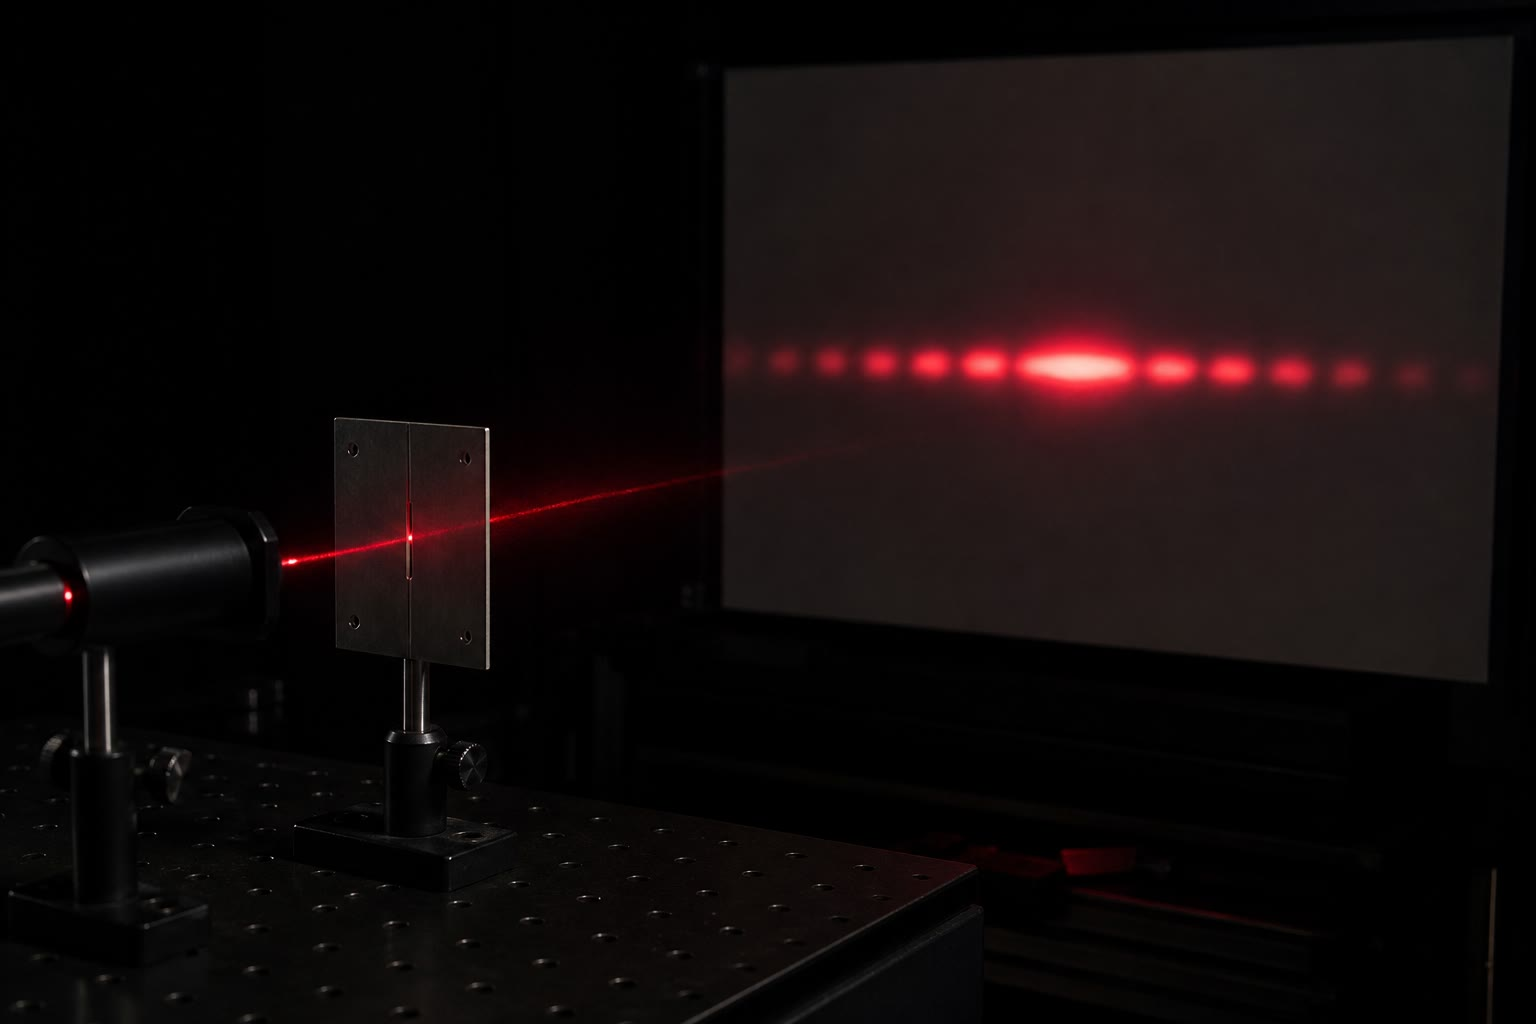
\includegraphics[width=0.58\linewidth]{images/book4/ai/b4-22-slit-diffraction-pattern.jpg}

{\small حزمة ليزر عبر شقّ ضيّق: على الشاشة البعيدة، الشريط المركزي المضيء العريض ومواضع العظم الجانبية الأخفت والأضيق في نقش فراونهوفر.}
\end{omfigure}

\section{مسألة: ما الذي يمكن تمييزه}

\begin{problem}[{مسألة نهاية الأسبوع --- حدّ الحيود على أربعة
سلالم: العين، والمقراب، والمجهر، وحزمة الليزر التي
يجب تنظيفها قبل استعمالها}]
\label{pb:b2:diffraction:1}

\medskip
\noindent\textbf{الجزء الأول --- العين.}
الحدقة $D = \qty{3}{mm}$ نهارًا، و \qty{7}{mm} ليلًا؛ و $\lambda = \qty{550}{nm}$؛ وتتباعد
مخاريط الشبكية \qty{2}{\micro m} في النقرة، والبعد البؤري
للعين \qty{17}{mm}.
\begin{enumerate}
  \item أوجد نصف القطر الزاوي \omterm{prop:b2:diffraction:airy}{لقرص إيري} نهارًا؛ ونصف قطره الخطي على
        الشبكية؛ وقارنه \omterm{def:b2:maxwell-equations:operators}{بتباعد} المخاريط --- أتكون الشبكية
        ملائمة للبصريات؟
  \item وأصغر فصل بين نقطتين يُميَّز على \qty{25}{cm}؛ وعلى
        \qty{10}{m}؛ أتستطيع قراءة نصّ \qty{1}{mm} على مدّ الذراع؟
  \item وتنفتح الحدقة ليلًا إلى \qty{7}{mm}: أوجد حدّ \omterm{def:b2:diffraction:huygens}{الحيود} عندئذ؛
        ولمَ يسوء البصر مع ذلك (بسبب زيغانات
        العدسة عند الفتحة الكاملة، والعصيّ أخشن من المخاريط)؟
  \item ومصباحا سيارة يبعد أحدهما عن الآخر \qty{1.5}{m}: أوجد المسافة التي
        يندمجان عندها في ضوء واحد.
  \item وثقب \qty{1}{mm} يُمسَك أمام العين: ماذا يفعل \omterm{def:b2:diffraction:huygens}{الحيود}،
        ولمَ يفيد ثقب الدبوس مع ذلك العين قصيرة النظر
        (بعمق الميدان)؟
\end{enumerate}

\medskip
\noindent\textbf{الجزء الثاني --- المقراب.}
مقراب \qty{1}{m}، و $f = \qty{10}{m}$، مع آلة تصوير ببكسلات \qty{10}{\micro m}؛
و $\lambda = \qty{550}{nm}$.
\begin{enumerate}[resume]
  \item أوجد حدّ \omterm{def:b2:diffraction:huygens}{الحيود} بالثواني القوسية؛ ونصف قطر إيري على
        الكاشف؛ وعدد البكسلات في \omterm{prop:b2:diffraction:airy}{قرص إيري}.
  \item ويشوّش الجوّ الصور إلى \qty{1}{''}: فكم يضيع من
        تمييز المقراب؟ وأوجد قطر المقراب الذي يتساوى عنده
        حدّ \omterm{def:b2:diffraction:huygens}{الحيود} مع الرؤية.
  \item وتصحّح البصريات التكيفية الجوَّ عند \qty{2.2}{\micro m}:
        أوجد حدّ \omterm{def:b2:diffraction:huygens}{الحيود} هناك؛ ولمَ يكون ذلك أيسر في تحت الأحمر؟
  \item ونجم ثنائي مركّبتاه متباعدتان \qty{0.15}{''}: أيُميَّز
        بالبصريات التكيفية عند \qty{2.2}{\micro m}؟ وعند \qty{550}{nm} من الفضاء؟
  \item والقمر على بعد \qty{3.8e5}{km}: أوجد أصغر فوّهة يستطيع هذا المقراب
        تمييزها (\omterm{def:b2:diffraction:huygens}{بالحيود} وحده)؛ وموطئ مركبة قمرية (\qty{4}{m})؟
  \item وقدرة المقراب على جمع الضوء بالنسبة إلى
        العين الليلية (\qty{7}{mm})؛ وماذا يشتري ذلك، وماذا لا يشتري؟
  \item وضوء نجم عبر الأذرع الأربعة الحاملة للمرآة
        الثانوية: صِف الصورة.
\end{enumerate}

\medskip
\noindent\textbf{الجزء الثالث --- المجهر.}
شيئية فتحتها العددية $\mathrm{NA} = n\sin\alpha = 0.9$ (جافّة) أو $1.4$
(بالزيت)، و $\lambda = \qty{550}{nm}$؛ والمسافة المميَّزة هي $0.61\lambda/\mathrm{NA}$.
\begin{enumerate}[resume]
  \item أوجد المسافة المميَّزة مع كل شيئية؛ وعدد أزواج الخطوط
        في المليمتر.
  \item وجرثومة \qty{1}{\micro m} فيها بنية داخلية عند
        \qty{0.2}{\micro m}: ماذا يُرى بكل منهما؟ وفيروس \qty{0.1}{\micro m}؟
  \item وآبي: لا تُصوَّر بنية دورية دورها $d$ إلا إذا دخلت
        رتبتاها الأوليان عند $\sin\theta = \lambda/d$ في الشيئية: أوجد أصغر $d$
        من أجل $\mathrm{NA} = 1.4$؛ وقارنه بالمقدار $0.61\lambda/\mathrm{NA}$.
  \item ولمَ يحسّن الزيت بين الشريحة والشيئية
        التمييز؟
  \item وفوق البنفسجي عند \qty{250}{nm} ومجهر إلكتروني عند \qty{4}{pm}:
        أوجد المسافتين المميَّزتين بالصيغة نفسها (وللإلكترونات تكون
        \omterm{prop:b2:guided-waves:fibre}{الفتحة العددية} العملية \qty{0.01}{}): قارن.
  \item والخلية شفافة: ففي الحقل المضيء تكون صورتها فارغة.
        فسّر في جملتين ما تفعله صفيحة تباين الطور في \omterm{prop:b2:diffraction:fourier}{مستوي
        فورييه} للشيئية.
\end{enumerate}

\medskip
\noindent\textbf{الجزء الرابع --- الحزمة.}
ليزر عند \qty{532}{nm}، وقطر حزمته \qty{1.5}{mm}، يُراد توسيعها إلى
\qty{30}{mm} وتنظيفها.
\begin{enumerate}[resume]
  \item أوجد نصف زاوية \omterm{def:b2:diffraction:huygens}{حيود} الحزمة الخام ($\sim1.22\lambda/D$)؛ وقطرها
        بعد \qty{100}{m} من دون بصريات.
  \item وعدسة $f_1 = \qty{10}{mm}$ تجمّعها: أوجد قطر البقعة البؤرية؛
        وقطر ثقب الدبوس المختار ($1.5\times$ البقعة).
  \item وعدسة ثانية $f_2$ تعيد التوازي عند \qty{30}{mm}: أوجد $f_2$؛ وزاوية
        \omterm{def:b2:diffraction:huygens}{الحيود} الجديدة؛ والقطر بعد \qty{1}{km}.
  \item وغبار \qty{100}{\micro m} على العدسة الأولى يحيد عند أي زاوية؛
        وأين يقع ذلك الضوء في مستوي الثقب، وماذا
        يحلّ به؟
  \item ويمرّر الثقب $99\%$ من حزمة غاوسية: أوجد الاستطاعة الضائعة، وأين
        تذهب.
  \item ولمَ يجب أن تكون الحزمة الموسَّعة \emph{أكبر} لتبقى متوازية
        (اربط $\lambda/D$ بالمسافة التي يتضاعف عليها قطر الحزمة،
        $\sim D^2/\lambda$)؟
  \item ولخّص حدود هذه المسألة الأربعة في جدول واحد: الفتحة،
        وطول الموجة، و $\lambda/D$، وما الذي يحدّه.
\end{enumerate}
\end{problem}
